\documentclass[a4paper,12pt]{article}

\RequirePackage{epsfig}
\usepackage{graphicx}
\usepackage[backend=biber,
            style=numeric,
            urldate=short,
            texencoding=utf8,
            bibencoding=utf8]
  {biblatex}
\addbibresource{ProjectPlan.bib}

\setlength\hoffset{-0.5in}      %% these work quite well with a 12pt font
\setlength\voffset{-0.5in}
\setlength{\textwidth}{6.30in}
\setlength{\textheight}{9.0in}


\begin{document}

\begin{center}
{\Large\bf{Dynamic Traffic Pricing Strategies using AI}} \\
      \vspace{4.0mm}
{\Large\bf{Project Plan}} \\
      \vspace{6mm}
      {\large\bf{Karlis Venters}}  \\
      \vspace{4.0mm}
       {\tt karlis.venters.10@abdn.ac.uk} \\
      \vspace{4.0mm}
      {\em Department of Computing Science,\\
       University of Aberdeen, Aberdeen AB24 3UE, UK} 
\end{center}


\section*{Introduction}
Taxicabs use taximeters to calculate their fares based on route distance and time spent travelling. However, the actual costs and potential profits are influenced by more factors. If fare prices were set dynamically, they would account for the actual environment and increase profitability of taxicabs. Usage of artificial intelligence (AI) has been successfully researched in \cite{tavares2012reinforcement} and \cite{ben2010road} for traffic routing, and in \cite{lou2011optimal} for variable pricing of toll lanes. A variable pricing approach for public transport fares is suggested in \cite{emele2013agent}. Therefore AI could be used to dynamically price taxicab fares.

\section*{Goals}
The project hypothesis is that taxicab profits can be improved by adapting a dynamic pricing strategy instead of charging fares calculated by a taximeter. The prices can be set by an AI system using reinforcement learning with increased profit being the ultimate goal. This hypothesis can experimentally be tested in a simulation of a transport network that consists of: a taxicab (agent) travelling in a network (graph) between destinations (vertices) that are connected with routes (edges), where the taxicab can transport a passenger between destinations in return for a fare. Taxicab offers a fare to a passenger, who in turn can agree or decline (losing the passenger if declined). Passengers are ready to pay a fare up to a sum that is function of the journey distance and other  characteristics such as passenger income and time of day. Thus the taxicab will learn to offer the right fares for maximised profits depending on environmental circumstances. If this experiment has been performed and evaluated, software is demonstrated and submitted on time and a report is written and submitted before the deadline, then this project can be deemed successful.
\section*{Additional extras} The basic model described above can be extended to be closer to the real world. For example, a simple extension is adding toll roads and toll destinations. Passengers could be modelled to take non-discrete actions to take in account other factors besides price, furthermore, passengers and taxicabs could haggle about the fare. There could be multiple passengers queuing at a location, who may agree to share the taxicab or bid on the taxi. Another feature of real transport networks is having multiple taxicabs, in this case the AI system will need to be modelled to be aware of them. They could be competing, or they may be working for the same company in which case the goal is overall profitability of all taxicabs in the company.

\section*{Methodology}
To ensure that the project is progressing successfully, there will be weekly meetings with supervisor. All work undertaken will be documented, continuously taking notes and writing relevant sections of the project submission. Software development and experiments will be iterative and incremental to accommodate the basic goals and any additional extras. The project has the following distinct stages:
\begin{itemize} 
\item Researching literature on AI and related works to model environment and choose an appropriate machine learning algorithm, writing a literature review and designing the experiment.
\item Designing and developing software, following Kanban project management framework and test driven development (TDD) practices. Both Kanban and TDD are widely accepted in software development industry and familiar to the author.
\item Running simulations both with a taximeter and with dynamic pricing approaches and gathering data.
\item Timely evaluation and writing up before deadline; and preparation for presentation.
\end{itemize}

\section*{Resources Required}
A modern computer running Java. Literature on AI and related research, project management and software development.

\section*{Risk Assessment}
The main risks are time-related, for example, more time is needed to develop software. These risks can be mitigated by following the timetable below that allows plenty of extra time. Another risk is technical human or computer error which can be mitigated by using source control, using cloud data storage and taking frequent backups.

\section*{Timetable}
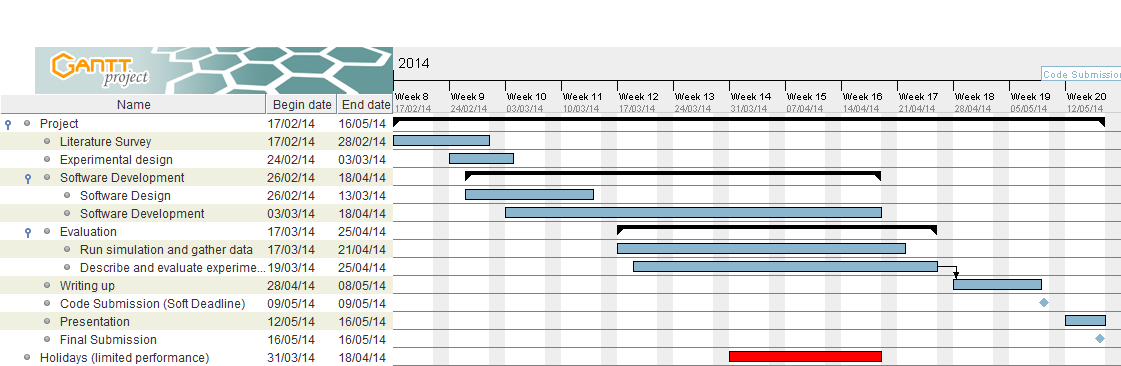
\includegraphics[width=\textwidth]{gantt}


\printbibliography

\end{document}
